\chapter{Conclusion}

\todo{first finish the whole thesis, then the intro and then come back to rewrite the first sentence}
We got almost $4$ orders of magnitude improvement in the relative error both in the \ac{UWF}\index{UWF}($n=64$, $m=640$, 
and in the unfolded $L=160$ times) and the \ac{URWF}\index{URWF}($n=64$, $m=640$, and unfolded $L=30$ times) after performing 
\ho \cite{Hutter2019}\cite{Akiba2019}\index{\hp} compared to the \ac{WF}\cite{Candes2014}\index{\ac{WF}} 
\cref{pseudocode:wf} and the \ac{RWF}\cite{Zhang2016}\index{\ac{RWF}} 
\cref{pseudocode:rwf} using the same number of iteration which can be seen in 
\cref{fig:proposed_winning_scenarios} which is a smaller sized version of \cref{fig:uwf_training_07_08_optuna} and 
in \cref{fig:proposed_winning_scenarios} which is a smaller sized version of \cref{fig:urwf_training_07_08_optuna}. The model is still 
interpretable thanks to the scenarios we considered as we were only focusing on tinkering with the step size and therefore 
the total structure of the iterative algorithm is intact(We did not change the innate nonlinearities associated with the algorithms). 
The datasets are very small(only $100$ samples) compared to today's \ml/\dl \cite{Goodfellow2016}\cite{LeCun2015} 
counterparts' \cite{Krizhevsky2017}\cite{Szegedy2014} datasets(millions of samples). Increasing the the number of samples from $100$ to $500$ resulted in almost 
no improvement in the relative error. In the proposed winning scenarios, different scalars multiplied by a single matrix of the form $\tau_k\boldsymbol{M}$, you only need to train 
$n^2+L$(around $4100$ for both the \ac{UWF} and the \ac{URWF}) parameters which tremendously reduces the required number of 
\ac{FLOPS}\cite{Hager2010}\cite{Hennessy2019}\index{\ac{FLOPS}} and in turn training time to reach satisfactory 
relative errors both on the train and the test data. If we were to use a fully connected multi-perceptron \nn we would have 
had, depending on the exact architecture, roughly $Lmn$(around $1.2$ million for the \ac{URWF} and around $6.5$ million for the \ac{UWF}) 
As another example to show the sheer size of the general contemporary \ml/\dl models and put that into perspective, 
ImageNet\cite{Deng2009}\index{ImageNet} has around $14$ millions images and a relatively new model like GoogleNet\cite{Szegedy2014}\index{GoogleNet}, 
depending on the instance that you use, has millions of parameters only to classify an image as one of the $1000$ 
classes. What got me very interested in taking \du/\au\cite{Monga2019} as my thesis topic was to go for \ml/\dl models with relatively few number of parameters 
rather than the general direction that is currently trending. If you are reading this, it is my hope that my work could 
somehow win you over and convince you that small does not always mean weak.


% \afterpage{%
%   \clearpage % Start a new page
\begin{figure}[!htbp]
    \captionsetup{justification=centering}
%   \subfloat[Different Matrices$(\boldsymbol{M}_k)$, $\mathrm{lr}=1.000\times10^{-3}, \,\mathrm{L}=30$]{% This file was created with tikzplotlib v0.10.1.
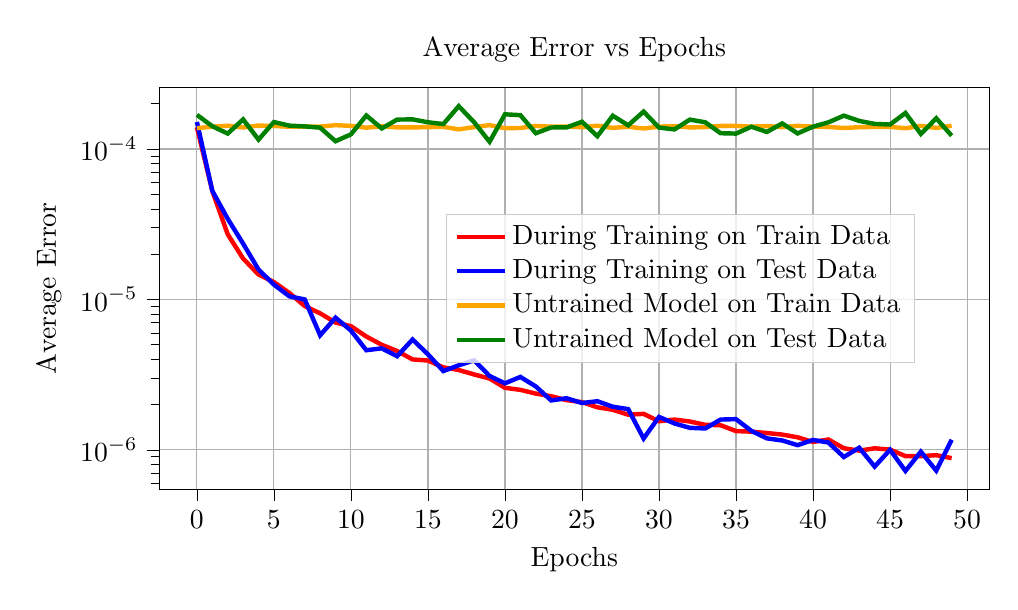
\begin{tikzpicture}

  \definecolor{darkgray176}{RGB}{176,176,176}
  \definecolor{green}{RGB}{0,128,0}
  \definecolor{lightgray204}{RGB}{204,204,204}
  \definecolor{orange}{RGB}{255,165,0}
  
  \begin{axis}[
    width = 1.0\textwidth,
    height = 19em,
  legend cell align={left},
  legend style={
    fill opacity=0.8,
    draw opacity=1,
    text opacity=1,
    at={(0.91,0.5)},
    anchor=east,
    draw=lightgray204
  },
  % log basis y={10},
  tick align=outside,
  tick pos=left,
  title={Average Error vs Epochs},
  x grid style={darkgray176},
  xlabel={Epochs},
  xmajorgrids,
  xmin=-2.45, xmax=51.45,
  xtick style={color=black},
  y grid style={darkgray176},
  ylabel={Average Error},
  ymajorgrids,
  ymin=5.47956319196448e-07, ymax=0.000254691381547786,
  ymode=log,
  ytick style={color=black},
  ytick={1e-08,1e-07,1e-06,1e-05,0.0001,0.001,0.01},
  yticklabels={
    \(\displaystyle {10^{-8}}\),
    \(\displaystyle {10^{-7}}\),
    \(\displaystyle {10^{-6}}\),
    \(\displaystyle {10^{-5}}\),
    \(\displaystyle {10^{-4}}\),
    \(\displaystyle {10^{-3}}\),
    \(\displaystyle {10^{-2}}\)
  }
  ]
  \addplot [ultra thick, red]
table {%
0 0.000139422554639168
1 5.25441355421208e-05
2 2.709246109589e-05
3 1.86883116839454e-05
4 1.4641495909018e-05
5 1.30382604766055e-05
6 1.10479877548642e-05
7 9.03117143025156e-06
8 8.08377171779284e-06
9 7.014934453764e-06
10 6.64117942505982e-06
11 5.66791140954592e-06
12 4.99323004987673e-06
13 4.53997472504852e-06
14 3.99270811612951e-06
15 3.92411902794265e-06
16 3.53491191162902e-06
17 3.39455823450407e-06
18 3.1713191219751e-06
19 2.97965834761271e-06
20 2.58465047409118e-06
21 2.5051617740246e-06
22 2.36605910686194e-06
23 2.27213763537293e-06
24 2.14105693885358e-06
25 2.07581410904822e-06
26 1.91861840903584e-06
27 1.84637030997692e-06
28 1.71315411989781e-06
29 1.73497676314582e-06
30 1.54966937770951e-06
31 1.59103592523024e-06
32 1.54397719143162e-06
33 1.46790443977807e-06
34 1.45789761063497e-06
35 1.33272737912193e-06
36 1.32122954710212e-06
37 1.2942375633429e-06
38 1.26361408092635e-06
39 1.21193875202152e-06
40 1.12860448098218e-06
41 1.17169065561029e-06
42 1.0251166031594e-06
43 9.8811494808615e-07
44 1.02411047464557e-06
45 1.00423574167507e-06
46 9.08802235244366e-07
47 9.08564288693015e-07
48 9.21839614420605e-07
49 8.81109031070082e-07
};
\addlegendentry{During Training on Train Data}
\addplot [ultra thick, blue]
table {%
0 0.000151191532495432
1 5.27330812474247e-05
2 3.43467727361713e-05
3 2.34825092775282e-05
4 1.57967224367894e-05
5 1.25444585137302e-05
6 1.04895107142511e-05
7 9.99405347101856e-06
8 5.77313267058344e-06
9 7.56428335080273e-06
10 6.20858509137179e-06
11 4.59601551483502e-06
12 4.72754800284747e-06
13 4.19237494497793e-06
14 5.41578947377275e-06
15 4.31831585956388e-06
16 3.34092874254566e-06
17 3.64814991371532e-06
18 3.93835989598301e-06
19 3.09812821797095e-06
20 2.76999890047591e-06
21 3.05379262499628e-06
22 2.63992797044921e-06
23 2.13079511013348e-06
24 2.2038937004254e-06
25 2.0483175831032e-06
26 2.10558482649503e-06
27 1.93491723621264e-06
28 1.86590375506057e-06
29 1.18982120511646e-06
30 1.65560504683526e-06
31 1.49886989220249e-06
32 1.40136648951739e-06
33 1.38726443310588e-06
34 1.5903664234429e-06
35 1.600476934982e-06
36 1.33635251131636e-06
37 1.19272579013341e-06
38 1.15448892756831e-06
39 1.07466962617764e-06
40 1.16404714844975e-06
41 1.11877704966901e-06
42 8.96443566489324e-07
43 1.03346019386663e-06
44 7.74358625221794e-07
45 1.00108979950164e-06
46 7.24411620467436e-07
47 9.72342604654841e-07
48 7.2755648261591e-07
49 1.16638921099366e-06
};
\addlegendentry{During Training on Test Data}
\addplot [ultra thick, orange]
table {%
0 0.000137548107886687
1 0.000140638832817785
2 0.000142808101372793
3 0.000138855073601007
4 0.00014315867156256
5 0.000142147371661849
6 0.000140535441460088
7 0.000140832271426916
8 0.000141012889798731
9 0.000143917815876193
10 0.000142426055390388
11 0.000138538351166062
12 0.000141437121783383
13 0.000139053459861316
14 0.000139040130306967
15 0.000139728872454725
16 0.000140273332362995
17 0.00013496758765541
18 0.000139760843012482
19 0.000144059871672653
20 0.000137425566208549
21 0.000137912458740175
22 0.000142265387694351
23 0.000140677715535276
24 0.000141052427352406
25 0.000139516676426865
26 0.00014278301387094
27 0.000138091811095364
28 0.000140507239848375
29 0.000136786737130024
30 0.00014075510262046
31 0.000142040196806192
32 0.000139078518259339
33 0.000139772397233173
34 0.000142270961077884
35 0.000142297969432548
36 0.000140746793476865
37 0.000141959739266895
38 0.000139722877065651
39 0.000142463482916355
40 0.000140872885822318
41 0.00014001976524014
42 0.000137886876473203
43 0.000139517200295813
44 0.00014015486522112
45 0.000140228410600685
46 0.000137308554258198
47 0.00014238734729588
48 0.000138002840685658
49 0.000142704491736367
};
\addlegendentry{Untrained Model on Train Data}
\addplot [ultra thick, green]
table {%
0 0.000168594866408966
1 0.000141678872751072
2 0.000126560087664984
3 0.000157214250066318
4 0.000115438073407859
5 0.000150999199831858
6 0.000142947799758986
7 0.000141304670250975
8 0.000138527931994759
9 0.000112627378257457
10 0.000125072823720984
11 0.000166890022228472
12 0.000136944450787269
13 0.000156815774971619
14 0.000157319751451723
15 0.000150483218021691
16 0.000146467093145475
17 0.00019265255832579
18 0.000150442734593526
19 0.000111669789475854
20 0.000169916238519363
21 0.000167860955116339
22 0.000127240127767436
23 0.000138955030706711
24 0.000139115072670393
25 0.000151672968058847
26 0.000121595592645463
27 0.000166218713275157
28 0.000143689205287956
29 0.000177146794158034
30 0.000138729737955146
31 0.000134799440274946
32 0.00015673965390306
33 0.000150496722199023
34 0.000127258579595946
35 0.000126562154036947
36 0.000140600168379024
37 0.000129729727632366
38 0.000147858329000883
39 0.000126872822875157
40 0.000140709613333456
41 0.000150389416376129
42 0.000166537720360793
43 0.000153616216266528
44 0.000146757418406196
45 0.000145377474837005
46 0.000173495995113626
47 0.000125866179587319
48 0.000159938761498779
49 0.000122543351608329
};
\addlegendentry{Untrained Model on Test Data}
\end{axis}

\end{tikzpicture}}\\  
%   \subfloat[Different Semi-Positive Definite Matrices$(\boldsymbol{S}_k)$, $\mathrm{lr}=1.000\times10^{-3}, \,\mathrm{L}=30$]{% This file was created with tikzplotlib v0.10.1.
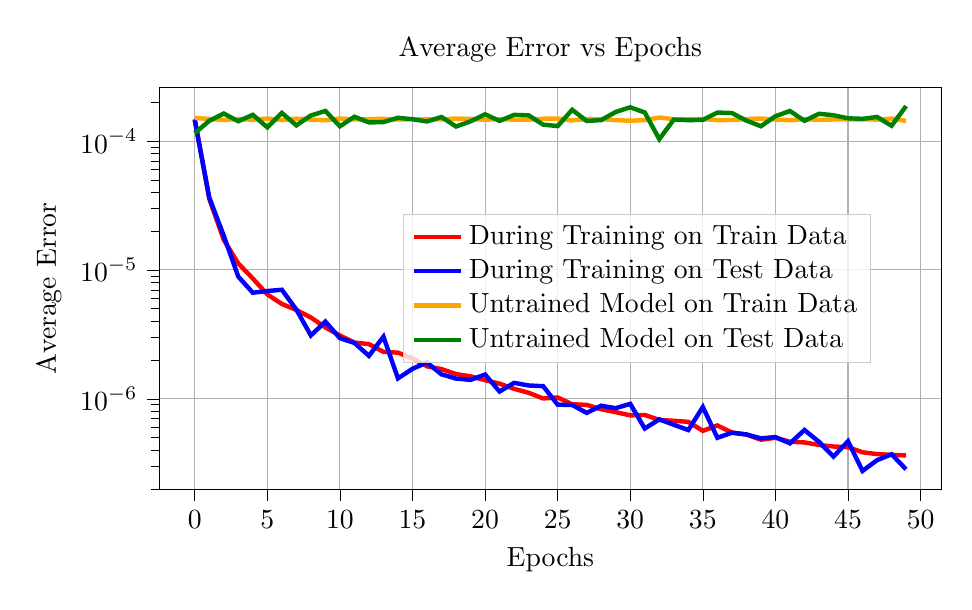
\begin{tikzpicture}

  \definecolor{darkgray176}{RGB}{176,176,176}
  \definecolor{green}{RGB}{0,128,0}
  \definecolor{lightgray204}{RGB}{204,204,204}
  \definecolor{orange}{RGB}{255,165,0}
  
  \begin{axis}[
    width = 0.95\textwidth,
    height = 19em,
  legend cell align={left},
  legend style={
    fill opacity=0.8,
    draw opacity=1,
    text opacity=1,
    at={(0.91,0.5)},
    anchor=east,
    draw=lightgray204
  },
  % log basis y={10},
  tick align=outside,
  tick pos=left,
  title={Average Error vs Epochs},
  x grid style={darkgray176},
  xlabel={Epochs},
  xmajorgrids,
  xmin=-2.45, xmax=51.45,
  xtick style={color=black},
  y grid style={darkgray176},
  ylabel={Average Error},
  ymajorgrids,
  ymin=1.98989848731464e-07, ymax=0.00025862395496495,
  ymode=log,
  ytick style={color=black},
  ytick={1e-08,1e-07,1e-06,1e-05,0.0001,0.001,0.01},
  yticklabels={
    \(\displaystyle {10^{-8}}\),
    \(\displaystyle {10^{-7}}\),
    \(\displaystyle {10^{-6}}\),
    \(\displaystyle {10^{-5}}\),
    \(\displaystyle {10^{-4}}\),
    \(\displaystyle {10^{-3}}\),
    \(\displaystyle {10^{-2}}\)
  }
  ]
  \addplot [ultra thick, red]
  table {%
  0 0.000148013044963591
  1 3.56593227479607e-05
  2 1.7092230336857e-05
  3 1.12235911728931e-05
  4 8.58035764395026e-06
  5 6.45710269964184e-06
  6 5.44462363905041e-06
  7 4.88857358504902e-06
  8 4.2726201172627e-06
  9 3.58169586434087e-06
  10 3.09524739350309e-06
  11 2.73389900939947e-06
  12 2.65521657638601e-06
  13 2.31281637752545e-06
  14 2.27968439503456e-06
  15 2.05286619348044e-06
  16 1.78653704097087e-06
  17 1.69934662608284e-06
  18 1.55517341227096e-06
  19 1.49384698033828e-06
  20 1.3938711163064e-06
  21 1.30992964386678e-06
  22 1.19467654258187e-06
  23 1.11279143766296e-06
  24 1.00586737517006e-06
  25 1.02330841400544e-06
  26 9.0733004753929e-07
  27 8.96316521448171e-07
  28 8.29465079732472e-07
  29 7.87274132107996e-07
  30 7.43528971725027e-07
  31 7.48820809803874e-07
  32 6.85715860981873e-07
  33 6.74960119795287e-07
  34 6.62006982565799e-07
  35 5.64021263471659e-07
  36 6.21000424416707e-07
  37 5.4747005151512e-07
  38 5.2761015467695e-07
  39 4.81172207855707e-07
  40 4.98232964218914e-07
  41 4.6397821051869e-07
  42 4.58541705938842e-07
  43 4.38037005778824e-07
  44 4.26196010039348e-07
  45 4.2150298895649e-07
  46 3.84383071150296e-07
  47 3.72081899513432e-07
  48 3.67385837307665e-07
  49 3.63334208941524e-07
  };
  \addlegendentry{During Training on Train Data}
  \addplot [ultra thick, blue]
  table {%
  0 0.000145961690577678
  1 3.6507273762254e-05
  2 1.83924421435222e-05
  3 8.87434453034075e-06
  4 6.65402694721706e-06
  5 6.85723716742359e-06
  6 7.01677663528244e-06
  7 4.92142953589791e-06
  8 3.10200198327948e-06
  9 3.96965651816572e-06
  10 2.95227073365822e-06
  11 2.71325984613213e-06
  12 2.15284285332018e-06
  13 3.03261163026036e-06
  14 1.43896522786235e-06
  15 1.70873647675762e-06
  16 1.90969149116427e-06
  17 1.54746635416814e-06
  18 1.43470697366865e-06
  19 1.4017372222952e-06
  20 1.54278404806973e-06
  21 1.13814337510121e-06
  22 1.32910520278529e-06
  23 1.26849226944614e-06
  24 1.25276187645795e-06
  25 9.00273789739003e-07
  26 8.95020548341563e-07
  27 7.7743254678353e-07
  28 8.83171367149771e-07
  29 8.45460078835458e-07
  30 9.13137625957461e-07
  31 5.87568308674236e-07
  32 6.92485286890587e-07
  33 6.28680254521896e-07
  34 5.71698194562487e-07
  35 8.63643435877748e-07
  36 4.98133147175395e-07
  37 5.44820807135693e-07
  38 5.29007309069129e-07
  39 4.93094887588086e-07
  40 5.04310378346418e-07
  41 4.50991336720108e-07
  42 5.72123838082916e-07
  43 4.63405569917086e-07
  44 3.56029943304748e-07
  45 4.6835725697747e-07
  46 2.75656987014372e-07
  47 3.33770287852531e-07
  48 3.71070939308993e-07
  49 2.83416682123061e-07
  };
  \addlegendentry{During Training on Test Data}
  \addplot [ultra thick, orange]
  table {%
  0 0.000151286862092093
  1 0.000148271938087419
  2 0.000145962316310033
  3 0.000148140708915889
  4 0.000146270336699672
  5 0.000149768020492047
  6 0.000145538549986668
  7 0.000149274768773466
  8 0.000146568301715888
  9 0.000144949066452682
  10 0.00014968030154705
  11 0.000146915088407695
  12 0.000148198654642329
  13 0.000148643390275538
  14 0.000147157494211569
  15 0.000147706436109729
  16 0.00014777151227463
  17 0.00014694788842462
  18 0.000149669518577866
  19 0.000148425155202858
  20 0.000146184596815147
  21 0.000148376799188554
  22 0.000146324280649424
  23 0.00014655634004157
  24 0.000149089726619422
  25 0.000149657396832481
  26 0.000144709527376108
  27 0.000148061357322149
  28 0.000147991930134594
  29 0.000145307276397943
  30 0.000143848243169487
  31 0.000145373909617774
  32 0.000152415770571679
  33 0.000147752347402275
  34 0.00014776736497879
  35 0.000147837854456156
  36 0.000145569443702698
  37 0.000145633559441194
  38 0.000148161940160207
  39 0.000149608822539449
  40 0.000146714635775425
  41 0.000145101090311073
  42 0.000147954560816288
  43 0.000146047284943052
  44 0.000147063998156227
  45 0.000147197628393769
  46 0.000147608181578107
  47 0.000146761129144579
  48 0.000149398503708653
  49 0.000143366807606071
  };
  \addlegendentry{Untrained Model on Train Data}
  \addplot [ultra thick, green]
  table {%
  0 0.000115061491669621
  1 0.000143547338666394
  2 0.000163512173458003
  3 0.000142517077620141
  4 0.000159814182552509
  5 0.00012783041165676
  6 0.000165362667758018
  7 0.000132426110212691
  8 0.000157876085722819
  9 0.000171300649526529
  10 0.000130172455101274
  11 0.000154473222210072
  12 0.000139474926982075
  13 0.000140412186738104
  14 0.000151597065269016
  15 0.00014767273387406
  16 0.000141933254781179
  17 0.000153813511133194
  18 0.000129606123664416
  19 0.000142261982546188
  20 0.000161294257850386
  21 0.00014334442676045
  22 0.000159681003424339
  23 0.000158348615514114
  24 0.000134108049678616
  25 0.000130705229821615
  26 0.000174892600625753
  27 0.000143100725836121
  28 0.000145519719808362
  29 0.000168184196809307
  30 0.000182958712684922
  31 0.000166574260219932
  32 0.000103557540569454
  33 0.000146681413752958
  34 0.000145311874803156
  35 0.00014605671458412
  36 0.000166460915352218
  37 0.000165033299708739
  38 0.000144075253047049
  39 0.000130360465846024
  40 0.000155840680235997
  41 0.000171156978467479
  42 0.000143605619086884
  43 0.000162815587827936
  44 0.000158585360622965
  45 0.000150236810441129
  46 0.000148762876051478
  47 0.000153807501192205
  48 0.000131454333313741
  49 0.000186694131116383
  };
  \addlegendentry{Untrained Model on Test Data}
  \end{axis}
  
  \end{tikzpicture}
  }\\  
\resizebox{1.0\textwidth}{!}{
  \subfloat[Proposed Winning Scenario for \ac{UWF} Using \optuna\cite{Akiba2019}\index{\optuna}: Different Scalars Multiplied by a Single Matrix$(\tau_k\boldsymbol{M})$, $\mathrm{lr}=8.798\times10^{-3}, \,\mathrm{L}=160$]{% This file was created with tikzplotlib v0.10.1.
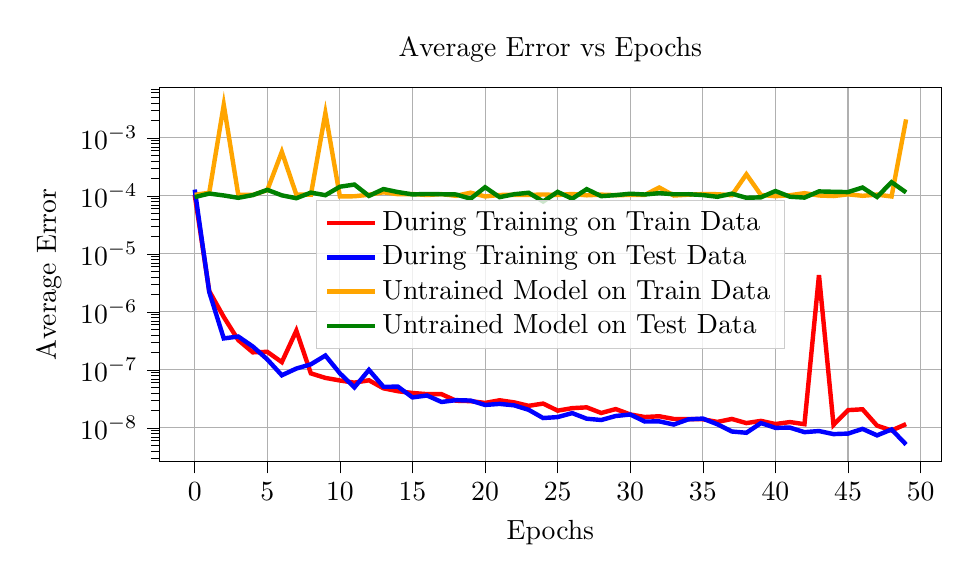
\begin{tikzpicture}

    \definecolor{darkgray176}{RGB}{176,176,176}
    \definecolor{green}{RGB}{0,128,0}
    \definecolor{lightgray204}{RGB}{204,204,204}
    \definecolor{orange}{RGB}{255,165,0}
    
    \begin{axis}[
      width = 0.95\textwidth,
      height = 18em,
    legend cell align={left},
    legend style={
      fill opacity=0.8,
      draw opacity=1,
      text opacity=1,
      at={(0.5,0.5)},
      anchor=center,
      draw=lightgray204
    },
    % log basis y={10},
    tick align=outside,
    tick pos=left,
    title={Average Error vs Epochs},
    x grid style={darkgray176},
    xlabel={Epochs},
    xmajorgrids,
    xmin=-2.45, xmax=51.45,
    xtick style={color=black},
    y grid style={darkgray176},
    ylabel={Average Error},
    ymajorgrids,
    ymin=2.63604330184737e-09, ymax=0.00725950156863836,
    ymode=log,
    ytick style={color=black},
    ytick={1e-10,1e-09,1e-08,1e-07,1e-06,1e-05,0.0001,0.001,0.01,0.1},
    yticklabels={
      \(\displaystyle {10^{-10}}\),
      \(\displaystyle {10^{-9}}\),
      \(\displaystyle {10^{-8}}\),
      \(\displaystyle {10^{-7}}\),
      \(\displaystyle {10^{-6}}\),
      \(\displaystyle {10^{-5}}\),
      \(\displaystyle {10^{-4}}\),
      \(\displaystyle {10^{-3}}\),
      \(\displaystyle {10^{-2}}\),
      \(\displaystyle {10^{-1}}\)
    }
    ]
    \addplot [ultra thick, red]
    table {%
    0 0.000104205340903718
    1 2.2795081804361e-06
    2 8.16013880466926e-07
    3 3.26127519656438e-07
    4 2.00797316551871e-07
    5 2.04524624791702e-07
    6 1.36023288632714e-07
    7 4.74071129019649e-07
    8 8.70571454925084e-08
    9 7.27430773395099e-08
    10 6.5652713487907e-08
    11 6.02018914719338e-08
    12 6.61969394855078e-08
    13 4.81310458155804e-08
    14 4.2873633532281e-08
    15 3.99703772302473e-08
    16 3.81714855279824e-08
    17 3.8142367486671e-08
    18 2.93974711240708e-08
    19 2.89232531258676e-08
    20 2.69239741612637e-08
    21 2.99225142441628e-08
    22 2.75352860512612e-08
    23 2.4009436216943e-08
    24 2.62635957426482e-08
    25 1.98318286237509e-08
    26 2.18844142807484e-08
    27 2.25979448487124e-08
    28 1.80841581709501e-08
    29 2.10961470514803e-08
    30 1.70547433953061e-08
    31 1.53920822754117e-08
    32 1.58656572324389e-08
    33 1.42510874212576e-08
    34 1.41820661880843e-08
    35 1.4081289023693e-08
    36 1.26731078964326e-08
    37 1.42557086135753e-08
    38 1.21001750841288e-08
    39 1.32015909315442e-08
    40 1.16595693100408e-08
    41 1.26017134505219e-08
    42 1.15926468424732e-08
    43 4.30966929343413e-06
    44 1.12703659738145e-08
    45 2.02334238252888e-08
    46 2.09316262100856e-08
    47 1.09466631315058e-08
    48 9.01701913136321e-09
    49 1.16273870531813e-08
    };
    \addlegendentry{During Training on Train Data}
    \addplot [ultra thick, blue]
    table {%
    0 0.000128205894725397
    1 2.19211028706923e-06
    2 3.48693362184349e-07
    3 3.7564521448985e-07
    4 2.53075398859437e-07
    5 1.51381684077023e-07
    6 8.07240780886787e-08
    7 1.05399159622266e-07
    8 1.24686110325456e-07
    9 1.76708667254388e-07
    10 8.71838210514397e-08
    11 4.9951530911585e-08
    12 9.98501263893559e-08
    13 5.1198544070985e-08
    14 5.13218765263446e-08
    15 3.35316165944732e-08
    16 3.61962158024198e-08
    17 2.79910761236124e-08
    18 3.00771283434642e-08
    19 2.95923321402825e-08
    20 2.4853880731257e-08
    21 2.59286903059319e-08
    22 2.44853541886414e-08
    23 2.05111181372786e-08
    24 1.47937218031302e-08
    25 1.5353929683215e-08
    26 1.79923898002698e-08
    27 1.44036702565131e-08
    28 1.36676279183234e-08
    29 1.603949861817e-08
    30 1.70154574874459e-08
    31 1.28716752811897e-08
    32 1.29476260823935e-08
    33 1.14277387552875e-08
    34 1.4037178530657e-08
    35 1.44796095113975e-08
    36 1.15444818149513e-08
    37 8.66101146357323e-09
    38 8.24099988250282e-09
    39 1.21144925202543e-08
    40 1.00226200672182e-08
    41 1.01044204114942e-08
    42 8.44652703335669e-09
    43 8.82723494299853e-09
    44 7.81588394005439e-09
    45 7.98052735007104e-09
    46 9.61182422543061e-09
    47 7.4352684009682e-09
    48 9.4029859454281e-09
    49 5.17222886742275e-09
    };
    \addlegendentry{During Training on Test Data}
    \addplot [ultra thick, orange]
    table {%
    0 0.000104004502645694
    1 0.000113090267404914
    2 0.00369982863776386
    3 0.000103595812106505
    4 0.000103680438769516
    5 0.000125327438581735
    6 0.000573276192881167
    7 0.000104799939435907
    8 0.000104467922938056
    9 0.00266967760398984
    10 9.74361173575744e-05
    11 9.83515856205486e-05
    12 0.000104475227999501
    13 0.000115149639896117
    14 0.000106749808765016
    15 0.000107450287032407
    16 0.000103390899312217
    17 0.000107067287899554
    18 0.000100105462479405
    19 0.000113200912892353
    20 9.77006420725957e-05
    21 0.000103448765003122
    22 0.000104000508144964
    23 0.000103353981103282
    24 0.000105591047031339
    25 0.000103221151221078
    26 0.00010765408660518
    27 0.000102091478765942
    28 0.000104882899904624
    29 0.000102825011708774
    30 0.000103528509498574
    31 0.000103895661595743
    32 0.000138981064083055
    33 0.000101232988527045
    34 0.000104792459751479
    35 0.000107034466054756
    36 0.000106611536466517
    37 0.000102448932011612
    38 0.000235152678214945
    39 0.000103626218333375
    40 9.85821752692573e-05
    41 0.000102437457826454
    42 0.000111155663034879
    43 0.000101380828709807
    44 9.91987908491865e-05
    45 0.000106175990367774
    46 0.000100137636763975
    47 0.000104896309494507
    48 9.75669390754774e-05
    49 0.00207684771157801
    };
    \addlegendentry{Untrained Model on Train Data}
    \addplot [ultra thick, green]
    table {%
    0 9.51192560023628e-05
    1 0.000109474291093647
    2 0.000101536650618073
    3 9.24414925975725e-05
    4 0.000102999874798115
    5 0.000126819082652219
    6 0.000101982383057475
    7 9.10065864445642e-05
    8 0.000113746289571282
    9 0.000102590936876368
    10 0.000143659664900042
    11 0.000156529058585875
    12 9.96770613710396e-05
    13 0.000130805958178826
    14 0.000116074705147184
    15 0.000105866813100874
    16 0.000107682615634985
    17 0.000106509614852257
    18 0.000105575592897367
    19 8.92794705578126e-05
    20 0.000140646734507754
    21 9.49161913013086e-05
    22 0.000106560277345125
    23 0.000113010035420302
    24 7.99219124019146e-05
    25 0.00011702597112162
    26 8.920714026317e-05
    27 0.000130467757117003
    28 9.88191241049208e-05
    29 0.000102830796095077
    30 0.000108744738099631
    31 0.000105451188574079
    32 0.000111337336420547
    33 0.000106409403088037
    34 0.000106660001620185
    35 0.000103220765595324
    36 9.62638878263533e-05
    37 0.000108933658339083
    38 9.25103668123484e-05
    39 9.42573096835986e-05
    40 0.000121093005873263
    41 9.66605221037753e-05
    42 9.32564653339796e-05
    43 0.000119190364785027
    44 0.000117450043035205
    45 0.0001160800238722
    46 0.000139031486469321
    47 9.57154188654386e-05
    48 0.000171932319062762
    49 0.000114621827378869
    };
    \addlegendentry{Untrained Model on Test Data}
    \end{axis}
    
    \end{tikzpicture}
    }\\  
% }
% \resizebox{0.67\textwidth}{!}{
  \subfloat[Proposed Winning Scenario for \ac{URWF} Using \optuna\cite{Akiba2019}\index{\optuna}: Different Scalars Multiplied by a Single Matrix$(\tau_k\boldsymbol{M})$, $\mathrm{lr}=7.622\times10^{-3}, \,\mathrm{L}=30$]{% This file was created with tikzplotlib v0.10.1.
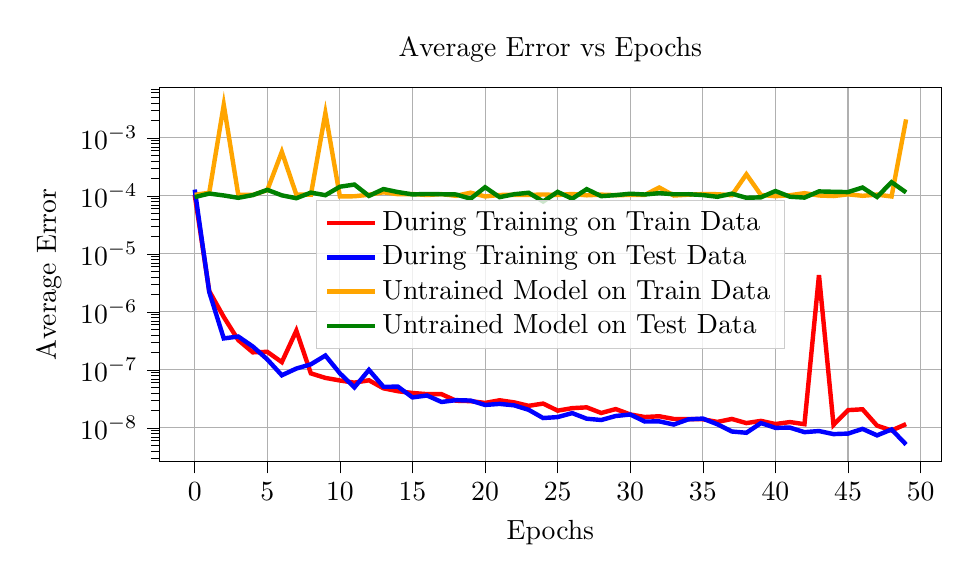
\begin{tikzpicture}

    \definecolor{darkgray176}{RGB}{176,176,176}
    \definecolor{green}{RGB}{0,128,0}
    \definecolor{lightgray204}{RGB}{204,204,204}
    \definecolor{orange}{RGB}{255,165,0}
    
    \begin{axis}[
      width = 0.95\textwidth,
      height = 18em,
    legend cell align={left},
    legend style={
      fill opacity=0.8,
      draw opacity=1,
      text opacity=1,
      at={(0.5,0.5)},
      anchor=center,
      draw=lightgray204
    },
    % log basis y={10},
    tick align=outside,
    tick pos=left,
    title={Average Error vs Epochs},
    x grid style={darkgray176},
    xlabel={Epochs},
    xmajorgrids,
    xmin=-2.45, xmax=51.45,
    xtick style={color=black},
    y grid style={darkgray176},
    ylabel={Average Error},
    ymajorgrids,
    ymin=2.63604330184737e-09, ymax=0.00725950156863836,
    ymode=log,
    ytick style={color=black},
    ytick={1e-10,1e-09,1e-08,1e-07,1e-06,1e-05,0.0001,0.001,0.01,0.1},
    yticklabels={
      \(\displaystyle {10^{-10}}\),
      \(\displaystyle {10^{-9}}\),
      \(\displaystyle {10^{-8}}\),
      \(\displaystyle {10^{-7}}\),
      \(\displaystyle {10^{-6}}\),
      \(\displaystyle {10^{-5}}\),
      \(\displaystyle {10^{-4}}\),
      \(\displaystyle {10^{-3}}\),
      \(\displaystyle {10^{-2}}\),
      \(\displaystyle {10^{-1}}\)
    }
    ]
    \addplot [ultra thick, red]
    table {%
    0 0.000104205340903718
    1 2.2795081804361e-06
    2 8.16013880466926e-07
    3 3.26127519656438e-07
    4 2.00797316551871e-07
    5 2.04524624791702e-07
    6 1.36023288632714e-07
    7 4.74071129019649e-07
    8 8.70571454925084e-08
    9 7.27430773395099e-08
    10 6.5652713487907e-08
    11 6.02018914719338e-08
    12 6.61969394855078e-08
    13 4.81310458155804e-08
    14 4.2873633532281e-08
    15 3.99703772302473e-08
    16 3.81714855279824e-08
    17 3.8142367486671e-08
    18 2.93974711240708e-08
    19 2.89232531258676e-08
    20 2.69239741612637e-08
    21 2.99225142441628e-08
    22 2.75352860512612e-08
    23 2.4009436216943e-08
    24 2.62635957426482e-08
    25 1.98318286237509e-08
    26 2.18844142807484e-08
    27 2.25979448487124e-08
    28 1.80841581709501e-08
    29 2.10961470514803e-08
    30 1.70547433953061e-08
    31 1.53920822754117e-08
    32 1.58656572324389e-08
    33 1.42510874212576e-08
    34 1.41820661880843e-08
    35 1.4081289023693e-08
    36 1.26731078964326e-08
    37 1.42557086135753e-08
    38 1.21001750841288e-08
    39 1.32015909315442e-08
    40 1.16595693100408e-08
    41 1.26017134505219e-08
    42 1.15926468424732e-08
    43 4.30966929343413e-06
    44 1.12703659738145e-08
    45 2.02334238252888e-08
    46 2.09316262100856e-08
    47 1.09466631315058e-08
    48 9.01701913136321e-09
    49 1.16273870531813e-08
    };
    \addlegendentry{During Training on Train Data}
    \addplot [ultra thick, blue]
    table {%
    0 0.000128205894725397
    1 2.19211028706923e-06
    2 3.48693362184349e-07
    3 3.7564521448985e-07
    4 2.53075398859437e-07
    5 1.51381684077023e-07
    6 8.07240780886787e-08
    7 1.05399159622266e-07
    8 1.24686110325456e-07
    9 1.76708667254388e-07
    10 8.71838210514397e-08
    11 4.9951530911585e-08
    12 9.98501263893559e-08
    13 5.1198544070985e-08
    14 5.13218765263446e-08
    15 3.35316165944732e-08
    16 3.61962158024198e-08
    17 2.79910761236124e-08
    18 3.00771283434642e-08
    19 2.95923321402825e-08
    20 2.4853880731257e-08
    21 2.59286903059319e-08
    22 2.44853541886414e-08
    23 2.05111181372786e-08
    24 1.47937218031302e-08
    25 1.5353929683215e-08
    26 1.79923898002698e-08
    27 1.44036702565131e-08
    28 1.36676279183234e-08
    29 1.603949861817e-08
    30 1.70154574874459e-08
    31 1.28716752811897e-08
    32 1.29476260823935e-08
    33 1.14277387552875e-08
    34 1.4037178530657e-08
    35 1.44796095113975e-08
    36 1.15444818149513e-08
    37 8.66101146357323e-09
    38 8.24099988250282e-09
    39 1.21144925202543e-08
    40 1.00226200672182e-08
    41 1.01044204114942e-08
    42 8.44652703335669e-09
    43 8.82723494299853e-09
    44 7.81588394005439e-09
    45 7.98052735007104e-09
    46 9.61182422543061e-09
    47 7.4352684009682e-09
    48 9.4029859454281e-09
    49 5.17222886742275e-09
    };
    \addlegendentry{During Training on Test Data}
    \addplot [ultra thick, orange]
    table {%
    0 0.000104004502645694
    1 0.000113090267404914
    2 0.00369982863776386
    3 0.000103595812106505
    4 0.000103680438769516
    5 0.000125327438581735
    6 0.000573276192881167
    7 0.000104799939435907
    8 0.000104467922938056
    9 0.00266967760398984
    10 9.74361173575744e-05
    11 9.83515856205486e-05
    12 0.000104475227999501
    13 0.000115149639896117
    14 0.000106749808765016
    15 0.000107450287032407
    16 0.000103390899312217
    17 0.000107067287899554
    18 0.000100105462479405
    19 0.000113200912892353
    20 9.77006420725957e-05
    21 0.000103448765003122
    22 0.000104000508144964
    23 0.000103353981103282
    24 0.000105591047031339
    25 0.000103221151221078
    26 0.00010765408660518
    27 0.000102091478765942
    28 0.000104882899904624
    29 0.000102825011708774
    30 0.000103528509498574
    31 0.000103895661595743
    32 0.000138981064083055
    33 0.000101232988527045
    34 0.000104792459751479
    35 0.000107034466054756
    36 0.000106611536466517
    37 0.000102448932011612
    38 0.000235152678214945
    39 0.000103626218333375
    40 9.85821752692573e-05
    41 0.000102437457826454
    42 0.000111155663034879
    43 0.000101380828709807
    44 9.91987908491865e-05
    45 0.000106175990367774
    46 0.000100137636763975
    47 0.000104896309494507
    48 9.75669390754774e-05
    49 0.00207684771157801
    };
    \addlegendentry{Untrained Model on Train Data}
    \addplot [ultra thick, green]
    table {%
    0 9.51192560023628e-05
    1 0.000109474291093647
    2 0.000101536650618073
    3 9.24414925975725e-05
    4 0.000102999874798115
    5 0.000126819082652219
    6 0.000101982383057475
    7 9.10065864445642e-05
    8 0.000113746289571282
    9 0.000102590936876368
    10 0.000143659664900042
    11 0.000156529058585875
    12 9.96770613710396e-05
    13 0.000130805958178826
    14 0.000116074705147184
    15 0.000105866813100874
    16 0.000107682615634985
    17 0.000106509614852257
    18 0.000105575592897367
    19 8.92794705578126e-05
    20 0.000140646734507754
    21 9.49161913013086e-05
    22 0.000106560277345125
    23 0.000113010035420302
    24 7.99219124019146e-05
    25 0.00011702597112162
    26 8.920714026317e-05
    27 0.000130467757117003
    28 9.88191241049208e-05
    29 0.000102830796095077
    30 0.000108744738099631
    31 0.000105451188574079
    32 0.000111337336420547
    33 0.000106409403088037
    34 0.000106660001620185
    35 0.000103220765595324
    36 9.62638878263533e-05
    37 0.000108933658339083
    38 9.25103668123484e-05
    39 9.42573096835986e-05
    40 0.000121093005873263
    41 9.66605221037753e-05
    42 9.32564653339796e-05
    43 0.000119190364785027
    44 0.000117450043035205
    45 0.0001160800238722
    46 0.000139031486469321
    47 9.57154188654386e-05
    48 0.000171932319062762
    49 0.000114621827378869
    };
    \addlegendentry{Untrained Model on Test Data}
    \end{axis}
    
    \end{tikzpicture}
    }\\  
}
  \caption{Proposed Winning Scenario for \ac{UWF} and \ac{URWF} after \HO Using \optuna\cite{Akiba2019}\index{\optuna}}
  \label{fig:proposed_winning_scenarios}
  \end{figure}
%   \clearpage % End the page
% }

